\documentclass{beamer}



%\usepackage{beamerthemesplit}
\usetheme{Boadilla}
%\usetheme{default}
%\useinnertheme{rounded}

%\useoutertheme{shadow}
\usecolortheme{rose}
%\usefonttheme{serif}
\setbeamertemplate{navigation symbols}{}
\usetheme{Madrid}

\usepackage{amssymb,amsmath,amscd,amsfonts,amsthm,dsfont,color,graphicx}
\usepackage{amscd}
%\usepackage[numbers]{natbib}
% \usepackage[french]{babel}
%\usepackage[active]{srcltx}


\def\qd{\,{\mathchar'26\mkern-12mu d}}

% \date[]{}

 \newcommand\makebeamertitle{\frame{\maketitle}}%

 \AtBeginDocument{
   \let\origtableofcontents=\tableofcontents
   \def\tableofcontents{\@ifnextchar[{\origtableofcontents}{\gobbletableofcontents}}
   \def\gobbletableofcontents#1{\origtableofcontents}
 }
\numberwithin{equation}{section}
  \theoremstyle{plain}
  \newtheorem*{thm*}{\protect\theoremname}
  \theoremstyle{plain}
  \newtheorem*{cor*}{\protect\corollaryname}
 \theoremstyle{definition}
 \newtheorem*{defn*}{\protect\definitionname}
 \theoremstyle{plain}
\newtheorem*{lem*}{\protect\lemmaname}
  \theoremstyle{plain}
  \newtheorem*{rem*}{\protect\remarkname}
   \theoremstyle{definition}
 \newtheorem*{prop*}{\protect\propositionname}

\usetheme{Madrid}

\makeatother

  \providecommand{\corollaryname}{Corollary}
  \providecommand{\definitionname}{Definitioninition}
  \providecommand{\theoremname}{Theorem}
   \providecommand{\lemmaname}{Lemma}
   \providecommand{\remarkname}{Remark}
   \providecommand{\propositionname}{Proposition}
   
   
   

\newcommand{\mbR}{\mathbb{R}}
\newcommand{\mbG}{\mathbb{G}}
\newcommand{\mbZ}{\mathbb{Z}}
\newcommand{\mbS}{S}

\newcommand{\brs}[1]{\left(#1\right)}
\newcommand{\set}[1]{\left\{#1\right\}}
\newcommand{\SqBrs}[1]{\left[#1\right]}
\newcommand{\clB}{\mathcal{B}}
\newcommand{\clF}{\mathcal{F}}
\newcommand{\clK}{\mathcal{K}}
\newcommand{\clL}{\mathcal{L}}
\newcommand{\clH}{\mathcal{H}}
\newcommand{\hilb}{\mathcal{H}}
\newcommand{\clS}{\mathcal{S}}
\newcommand{\abs}[1]{\left|#1\right|}
\newcommand{\tr}{{\rm Tr}}
\newcommand{\anglb}[1]{\langle#1\rangle}
\newcommand{\Vol}{\mathrm{Vol}}
\newcommand{\Rl}{\mathbb{R}}
   
\begin{document}

\title[The Dixmier trace and the DOS]{The Dixmier trace and the Density of States}


\author[E. McDonald]{Ed McDonald\\
Based on joint work with N. Azamov, E. Hekkelman F. Sukochev and D. Zanin.}

% Abstract: The Dixmier trace has been employed by Connes for several purposes, including defining the integral in noncommutative geometry. Connes' integration formula can be viewed as a way of associating a measure to a self-adjoint operator. In solid state physics there is another celebrated measure associated with Schrodinger operators: the density of states. Using techniques from noncommutative geometry, we have recently proved that the density of states can in many cases be computed by a Dixmier trace. This work also provides a new perspective on Roe's index theorem for open manifolds by giving a Dixmier trace formula for the index. Joint work with N. Azamov, E. Hekkelman, F. Sukochev and D. Zanin. 


\institute[]{Penn State University}

\makebeamertitle


\begin{frame}{Introduction}
This talk is about a connection between the density of states and Dixmier traces, covered in the two papers
\begin{itemize}
\item{} Azamov, M., Sukochev. and Zanin \emph{A Dixmier Trace Formula for the Density of States} Comm. Math. Phys. 377 (2020), no. 3, 2597–2628.  \texttt{arXiv:1910.12380}.
\item{} Azamov, Hekkelman, M., Sukochev and Zanin. \emph{An application of singular traces to crystals and percolation.} J. Geom. Phys. 179 (2022), Paper No. 104608, 22 pp. \texttt{arXiv:2202.03676}.
\end{itemize}
and the recent preprint
\begin{itemize}
\item{} Hekkelman and M. \emph{A general Dixmier trace formula for the density of states on open manifolds} (2023) \texttt{arXiv:2304.13272}.
\end{itemize}

% 
% Suppose that we are given a Schr\"odinger operator
% $$
%    H = - \Delta + V(x),
% $$
% where $V$ is a bounded measurable real-valued function.\\
% 
% Under suitable conditions, we have
% $$
%     \tr_\omega(f(H)(1+M_{|x|}^2)^{-\frac{d}{2}}) = \frac{\Vol(S^{d-1})}{d}\int_{\Rl} f\,d\nu_{H} 
% $$
% where $\nu_H$ is the density of states (DOS) measure for $H$.\\
% 
% (Of course I will explain what these notations mean!!)

% With $H$ one can associate a measure, $\nu_H,$ on the essential spectrum, $\sigma_{ess},$ of $H,$ which is called the density of states, as follows.
% 
% Take the restriction, $H_L,$ of $H$ to a cube, $\Omega_L := (-L,L)^d,$ of side length $2L$ with the centre at the origin, with domain $C^\infty_c(\Omega_L).$
% This restriction is a symmetric operator but not (essentially) self-adjoint. To make it essentially self-adjoint, we have to choose some boundary conditions.

\end{frame}

\begin{frame}{Introduction}
    Dixmier traces are best known due to their use by Connes to define the integration functional in noncommutative geometry. In particular, Connes gave a formula for the Hochschild class of the Chern character in terms of the Dixmier trace. \\
    \pause
    But their use is not limited to NCG. Today I will talk about one Dixmier trace formula which is meaningful in mathematical physics. \\
    \pause
    This formula was conjectured and proved on the basis of developments in NCG.
\end{frame}

\section{Dixmier trace formula for the density of states}

\begin{frame}
    \huge{Section 1: The density of states of Schr\"odinger operators}
\end{frame}
% 
\begin{frame}{The fundamental problem}
    If $H$ is a lower-bounded self-adjoint operator (on a Hilbert space) with discrete spectrum (i.e. the spectrum consists only of eigenvalues of finite multiplicity), then we can understand the spectrum through the spectral counting function
    \begin{align*}
        N(t,H) &= \tr(\chi_{(-\infty,t]}(H))\\
                     &= \text{ Dimension of the span of the eigenvectors}\\
                     &\text{ corresponding to eigenvalues }\leq t.
    \end{align*}
    \pause
    This is less useful when $H$ the spectrum of $H$ is not discrete. What is a good replacement?\pause


%     Let $F$ be a locally integrable function on $\Rl^d$, $d \geq 1$. A reasonable definition of a \emph{mean value} for $F$ is to take the limit
%     \begin{equation*}
%         \lim_{R\to\infty} \frac{1}{\Vol(B(0,R))}\int_{B(0,R)} F(t)\,dt
%     \end{equation*}
%     where $B(0,R)$ denotes the ball of radius $R>0$. Optimistically, this limit exists and defines a ``mean"
%     \begin{equation*}
%         m\{F\} := \lim_{R\to\infty} \frac{1}{\Vol(B(0,R))} \int_{B(0,R)}F(t)\,dt.
%     \end{equation*}
%     In general the limit may not converge, and instead a weak$^*$-limit point of the functionals $\{\frac{1}{\Vol(B(0,R))}\int_{B(0,R)}\}_{R>0}$
%     needs to be taken.
\end{frame} 
% 
% \begin{frame}{The Roe index theorem}
%     Let $M$ be a $d$-dimensional Riemannian spin manifold with spin bundle $S\rightarrow M$, and Dirac operator
%     $D$.
%     \pause
%     The local index theorem states that for all $p\in M$ we have
%     \begin{equation*}
%         \lim_{t\to 0} \Str(e^{-tD^2})(p,p) = \widehat{A}(R)(p)
%     \end{equation*}
%     where $\widehat{A}(R)$ is the (appropriately normalised) $\widehat{A}$-genus.
%     For any 
% \end{frame}


\begin{frame}{Physical setting}
    Initially we concentrate on Schr\"odinger operators.

    Let $d > 1$ and $R > 0$. Let $B(0,R)$ be the open ball in $\Rl^d$ of radius $R,$
    \begin{equation*}
        B(0,R) = \{x\in \Rl^d\;:\;|x|<R\}.
    \end{equation*}
    \pause
    On $L_2(B(0,R)),$ we can define the Dirichlet Laplace operator with Dirichlet boundary conditions, $\Delta_R.$
\end{frame}

\begin{frame}{Physical setting}
    The operator $\Delta_R$ is negative semidefinite and has purely discrete spectrum.\\
    \begin{center}
    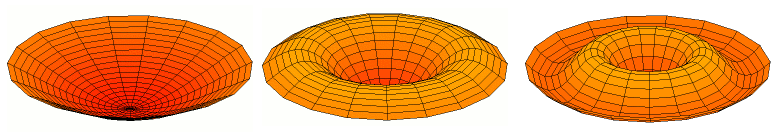
\includegraphics[width=110mm]{vibrating_drum.png}
    \end{center}
    As $R\to\infty,$ $N(t,-\Delta_R) \sim R^d.$
\end{frame}

\begin{frame}{Schr\"odinger operators on bounded domains}
    Given $V \in L_\infty(B(0,R))$, denote by $M_V$ the operator of pointwise multiplication by $V$. That is, $(M_V\xi)(t) = V(t)\xi(t)$. \pause \\
    For the purposes of this talk a \emph{Schr\"odinger operator} on $B(0,R)$ is a linear operator
    $$
        H = -\Delta_R+M_V
    $$
    where $V$ is real-valued. Since we only consider bounded $V$, the operator $H$ is self-adjoint with domain equal to that of $\Delta_R$.\pause
    
    Since $H$ is a relatively compact
    perturbation of $-\Delta_R$, the spectrum of $H$ is discrete and consists only of eigenvalues of finite multiplicity. 
\end{frame}

\begin{frame}{Schr\"odinger operators on $\Rl^d$}
    So far we have only discussed operators on bounded domains. What about unbounded domains?
    Let $\Delta = \sum_{j=1}^d \partial_{x_j}^2$ be the Laplace operator on $L_2(\Rl^d)$. This operator is self-adjoint,
    has spectrum $(-\infty,0]$ and has no eigenvalues. \pause We consider the Hamiltonian 
    $$
        H = -\Delta+M_V
    $$
    where $V \in L_\infty(\Rl^d)$ is real-valued.
    
    What does the spectrum of $H$ look like?  \pause
    The spectral counting function usually does not make sense for Schr\"odinger operators on $\Rl^d$, since the spectrum can be continuous.
\end{frame}

\begin{frame}{The density of states}
    What is a good replacement?\\
    \pause
    {\bf Idea}: (From solid-state physics.) Let $R > 0$, and ``restrict" $H$ to $B(0,R).$ Let
    \[
        H_R := -\Delta_R + M_{V}
    \]
    on $L_2(B(0,R))$. The \emph{density of states} of $H$ is a measure $\nu_H$ on $\Rl$ defined as
    \[
        \nu_H((-\infty,t]) := \lim_{R\to \infty} \frac{N(t,H_R)}{\mathrm{Vol}(B(0,R))},\quad t \in \Rl.
    \] 
    Optimistically, this limit exists and indeed defines a measure. 
\end{frame}

\begin{frame}{Problems with the density of states}
    There are many analytical issues with the ``measure" $\nu_H$.
    \begin{itemize}
        \item{} Does the limit as $R\to\infty$ really exist and does it define a measure? \pause    Answer: Not always, but sometimes it does. \pause
        \item{} If it exists, what is the support of $\nu_H$? \pause   Answer: the essential spectrum of $H$. \pause
        \item{} Does $\nu_H$ depend on the choice of boundary conditions for $H_R$? \pause   Answer: No. \pause
        \item{} Does it matter that we ``restricted" $H$ to balls $B(0,R)$? What about cubes or other domains? \pause Answer: For many classes of potentials $V$ (random, almost periodic), the choice of domain is irrelevant. For arbitrary potentials, the domain matters.
    \end{itemize}
\end{frame}

\begin{frame}{Example}
    An example where the DOS is easily computed is the ``free" Hamiltonian, corresponding to $V = 0$. We have
    \begin{equation*}
        \frac{d\nu_{-\Delta}}{dt} = \frac{\Vol(S^{d-1})}{2(2\pi)^d}\max\{t,0\}^{\frac{d}{2}-1}.
    \end{equation*}
\end{frame}


\begin{frame}{Insensitivity to localised perturbations}
    One of the important features of the DOS is that $\nu_{-\Delta+M_V}$ only cares about the behaviour of $V$ ``at infinity".\pause
    
    For example, if $V_1,V_0 \in L_{\infty}(\Rl^d)$ are such that $V_1-V_0$ is compactly supported, then 
    \[
        \nu_{-\Delta+M_{V_1}}=\nu_{-\Delta+M_{V_0}}.
    \]
    (assuming that both measures exist, of course.)
\end{frame}


% \begin{frame}{Questions about the density of states}
%     There has been a lot of research into the theoretical properties of $\nu_H$, with a particular emphasis on regularity of the ``integrated density of states"
%     $I_H(\lambda) := \nu_{H}((-\infty,\lambda]).$\pause
%     \begin{itemize}
%         \item{} The density of states has been proved to exist for some appropriate classes of ``random" potentials, e.g. 
%         \begin{equation*}
%             V(x) = \sum_{n\in \mathbb{Z}^d} \xi_n\phi(x-n),\quad x \in \mathbb{R}^d
%         \end{equation*}
%         where $\phi\in C^\infty_c(\Rl^d)$ and $\{\xi_n\}_{n\in \mathbb{Z}^d}$ are i.i.d. symmetrically distributed random variables.\pause
%         \item{} If $V$ is smooth and almost periodic, then $\nu_H$ exists.\pause
%         \item{} Under very mild conditions, $I_H$ is continuous.
%     \end{itemize}
% \end{frame}

\begin{frame}{Traces}
    Let $\mathcal{H}$ be a Hilbert space. An eigenvalue sequence of a compact operator $A\in B(\mathcal{H})$ is a sequence $\{\lambda(k,A)\}_{k\in \mathbb{N}}$ of the eigenvalues of $A$ listed with multiplicity, such that $\{\abs{\lambda(k,A)}\}_{k\in \mathbb{N}}$ is non-increasing.
    \bigskip
    
    The usual operator trace $\tr$ can be characterised for trace class operators $A\in \mathcal{L}_1 \subset B(\mathcal{H})$ as \[\tr(A) = \lim_{n\to \infty} \sum_{k=1}^n \lambda(k,A). \] 
\end{frame}
% 
% 
%     
% \begin{frame}{Ideals of compact operators}
%     Now for something completely different. \\ \pause
%     Let $\mathcal{H}$ be a Hilbert space. If $T$ is a compact operator on $H$, the singular value sequence of $T$ is defined as
%     $$
%         \mu(k,T) := \inf\{\|T-R\|_{\mathrm{op}}\;:\;\mathrm{rank}(R)\leq k\},\quad k\geq 0.
%     $$
%     (Equivalently, $\mu(T) = \{\mu(k,T)\}_{k=0}^\infty$ is the sequence of eigenvalues of the absolute value $|T|$ arranged in non-increasing order with multiplicities.)
%     
% \end{frame}
% 
% \begin{frame}{The trace class}
%     There is a well-developed theory (the \emph{Calkin correspondence}) which relates unitarily invariant ideals of compact operators
%     with rearrangement invariant sequence spaces. 
%     The trace class, $\mathcal{L}_1$, corresponds to those operators $T$ such that $\sum_{k=0}^\infty \mu(k,T) < \infty.$\pause
%     \begin{definition}
%         If $T\geq 0$ is trace class, the \emph{classical trace} $\tr$ is defined as
%         $$
%             \tr(T) = \sum_{k=0}^\infty \mu(k,T).
%         $$
%     \end{definition}
%     \pause
%     It is a theorem that $\tr$ extends to a continuous linear functional on $\mathcal{L}_1$, and obeys the tracial property
%     $$
%         \tr(AB) = \tr(BA),\quad A \in \mathcal{L}_1,\,B \in \mathcal{B}(H).
%     $$
%     \pause
%     Are there any other functionals with these properties?
% \end{frame}
%     
\begin{frame}{The weak trace class}
    A compact operator $T$ is said to be weak trace-class ($T \in \mathcal{L}_{1,\infty}$) if $\mu(k,T) = \mathcal{O}(k^{-1})$. Equivalently,
    $$
        \|T\|_{1,\infty} := \sup_{k\geq 0}\;(1+k)\lambda(k,|T|) < \infty.
    $$
    The class $\mathcal{L}_{1,\infty}$ is an an ideal.    
\end{frame}

\begin{frame}{Dixmier traces}
    The ideal $\mathcal{L}_{1,\infty}$ admits traces. That is, there exist nontrivial unitarily invariant functionals on $\mathcal{L}_{1,\infty}$.\\
    \pause
    An important class of examples are the famous Dixmier traces.\\
    If $T \in \mathcal{L}_{1,\infty}$, then
    \begin{equation*}
        \sum_{k=0}^N \lambda(k,T) = \mathcal{O}(\log(N)),\quad N\to\infty.
    \end{equation*}
    \pause
    An extended limit is a linear functional $\omega \in \ell_{\infty}(\mathbb{N})^*$
    which coincides with the ``limit" functional on the subspace of convergent sequences.\\
    If $T \geq 0$ is a positive element of $\mathcal{L}_{1,\infty}$, define $\tr_{\omega}(T)$
    as
    $$
        \tr_\omega(T) = \omega\left(\left\{\frac{1}{\log(2+N)}\sum_{k=0}^N \mu(k,T)\right\}_{N=0}^\infty\right).
    $$
\end{frame}

% \begin{frame}{Dixmier traces (cont.)}
%     It is a theorem that $\tr_{\omega}$ extends to a continuous linear unitarily invariant functional on $\mathcal{L}_{1,\infty}$. 
%     \begin{theorem}
%         If $0\leq T,S \in \mathcal{L}_{1,\infty}$, then $\tr_{\omega}(T+S) = \tr_\omega(T)+\tr_\omega(S).$\\
%         \pause
%         $\tr_\omega$ extends to a linear functional on $\mathcal{L}_{1,\infty}$ obeying the \emph{tracial} property
%         \begin{equation*}
%             \tr_\omega(BA) = \tr_\omega(AB),\quad A\in \mathcal{L}_{\infty},\,B \in \mathcal{L}_{1,\infty}.
%         \end{equation*}
%     \end{theorem}
%     \pause
%     There are other traces on $\mathcal{L}_{1,\infty}$, in fact there are $2^{|\mathbb{R}|}$ linearly independent traces.\\
%     These are highly singular, non-constructive objects.
% \end{frame}


\begin{frame}{Connes' integral formula}
    A property of Dixmier traces (and all traces on $\mathcal{L}_{1,\infty}$) is that they vanish on finite rank operators.
    \pause
    It was probably Connes whose realised that this property makes Dixmier traces computable in many situations. (One version of) Connes' integral formula states that
    if $f \in C^\infty_c(\Rl^d)$ then
    $$
        \tr_{\omega}(M_f(1-\Delta)^{-\frac{d}{2}}) = \frac{\Vol(S^{d-1})}{d(2\pi)^d}\int_{\Rl^d} f(t)\,dt.
    $$     
    This is taking place on the Hilbert space $\mathcal{H} = L_2(\Rl^d)$, and relies on the fact that $M_f(1-\Delta)^{-\frac{d}{2}} \in \mathcal{L}_{1,\infty}.$
\end{frame}

% 
% \begin{frame}{Computation formulae for Dixmier traces}
%     Surprisingly, Dixmier traces are often computable. \pause
%     \begin{theorem}[Zeta-function characterisation of the Dixmier trace]
%         Let $0 \leq A\in \mathcal{L}_{1,\infty}$ and let $B$ be a bounded operator. If
%         \begin{equation*}
%             \lim_{s\to 1} (s-1)\tr(BA^s) = c
%         \end{equation*}
%         if and only if for all extended limits $\omega$, we have
%         \begin{equation*}
%            \tr_\omega(BA) = c. 
%         \end{equation*}
%     \end{theorem}
%     \pause
%     Countless variations of this theorem exist, involving slightly different assumptions and different classes of traces on $\mathcal{L}_{1,\infty}$.
%     \pause
%     This is \emph{not} true under the weaker assumption that $BA \in \mathcal{L}_{1,\infty}$.
% \end{frame}

\begin{frame}{Connes' integral formula reconsidered}
    Restrict attention to a function $f \in C^\infty_c(\Rl^d)$ which is radial. There exists $g \in C_0([0,\infty))$ such that $f(t) = g(|t|^2)$. Then Connes' integral formula implies
%     \begin{align*}
%         \tr_{\omega}(M_f(1-\Delta)^{-\frac{d}{2}}) &= \frac{\Vol(S^{d-1})}{d(2\pi)^d} \int_{\Rl^d} g(|t|^2)\,dt\\
%                                                    &= \frac{\Vol(S^{d-1})^2}{2d(2\pi)^d}\int_{0}^\infty g(r)r^{\frac{d}{2}-1}\,dr. 
%     \end{align*}
    Switch to the Fourier side (recall that $\tr_{\omega}$ is unitarily invariant!) and we get
    $$
        \tr_{\omega}(g(-\Delta)(1+M_{|x|}^2)^{-\frac{d}{2}}) = \frac{\Vol(S^{d-1})}{d}\int_0^{\infty} g(r) \,d\mu(r)
    $$
    where $\mu$ is the measure $d\mu(r) = \frac{\Vol(S^{d-1})}{2(2\pi)^d}r^{\frac{d}{2}-1}\,dr.$
     
    This measure $\mu$ is precisely the density of states measure for the ``free" Hamiltonian $H = -\Delta$. This is not a coincidence!
\end{frame}

\begin{frame}{Idea of the formula}
    Idea: Replace $-\Delta$ with $H = -\Delta+M_V$. An argument using the Riesz representation theorem implies that there exists a measure $\mu_H$ on $\Rl$ such that 
    $$
        \tr_{\omega}(f(H)(1+M_{|x|}^2)^{-\frac{d}{2}}) = \frac{\Vol(S^{d-1})}{d}\int_{\Rl} f\,d\mu_H
    $$
    for all $f \in C_c(\Rl).$\\
    
    \begin{theorem}
        $\nu_H = \mu_H$.\\
        
        That is, if the density of states measure $\nu_H$ exists, then it is given by the formula
        $$
            \tr_{\omega}(f(H)(1+M_{|x|}^2)^{-\frac{d}{2}}) = \frac{\Vol(S^{d-1})}{d}\int_{\Rl} f\,d\nu_H,\quad f \in C_c(\Rl).
        $$
    \end{theorem}
\end{frame} 


\begin{frame}{Advantages of the Dixmier trace formula for DOS}

1. Simplifies proofs of some properties of DOS, such as insensitivity to localised perturbations described above.\\

2. Makes some computations very easy. For example, when $V$ is radially homogeneous (i.e., $V(r\xi) = V(\xi)$ for all $r>0$). In this case, the DOS exists and
    \[
        \frac{d\nu_{-\Delta+M_V}}{dt} = \frac{\Vol(S^{d-1})}{2(2\pi)^d}\cdot \left(\frac{1}{\mathrm{Vol}(S^{d-1})}\int_{S^{d-1}} \max\{t-V(\theta),0\}^{\frac{d}{2}-1}\,d\theta\right).
    \]
    See N.~Azamov, E.~M., F.~Sukochev and D.~Zanin \emph{The density of states depends on the domain} Oper. Matrices \textbf{16}, No. 4 (2022), 1185--1189 \texttt{arXiv:2107.09828}.
\end{frame}


\section{Recent developments}
\begin{frame}
    \huge{Section 2: Recent developments}
\end{frame}


\begin{frame}{Trace formulas}
    Our original proof in 2020 of the Dixmier trace formula for the DOS was concerned only with Schr\"odinger operators on $\Rl^n,$ and relied heavily on these assumptions.\pause

    Since then, we have made a lot of progress in understanding why the formula is true and we have several generalisations.\pause

    In particular:
    \begin{enumerate}
        \item{} The underlying space does not need to be Euclidean\pause
        \item{} The operator does not need to be Schr\"odinger operator.
    \end{enumerate}

\end{frame}
    
\begin{frame}{A general theorem}
    If $(X,d_X)$ is a measure space equipped with a Borel measure $\mu,$ and $H$ is an operator on $L_2(X,\mu),$ we can define a density of states for $H$ in a similar way to how it was defined for Schr\"odinger operators on $\Rl^d.$
        
    \begin{block}{General form}
    Let $(X, d_X)$ be a metric space equipped with a measure $\mu$ \emph{satisfying certain assumptions}. Let $H$ be a self-adjoint operator on $L_2(X)$ \emph{satisfying certain assumptions} for which the DOS $\nu_H$ exists \emph{in some particular sense}. Then for a certain (fixed) function $w\in L_\infty(X)$ and for all Dixmier traces $\tr_\omega$ and for all $f \in C_c(\mathbb{R})$ we have
    \begin{equation*}\label{F: DOS integral}
        \tr_\omega(f(H)M_w) = c\int_{\mathbb{R}} f\,d\nu_H.
    \end{equation*}
    where $c$ is a constant depending on $w$ but not $H$ or $f.$
    \end{block}
\end{frame}




\begin{frame}
We have proved this theorem in two different settings, using totally different methods.

\begin{block}{Azamov--Hekkelman--M.--Sukochev--Zanin (2022)}
$X$ a discrete metric space with some geometrical conditions, $H$ a general self-adjoint operator, $w(x) = \frac{1}{1+|B(x_0, d_X(x_0, x))|}$.
\end{block}

\begin{block}{Hekkelman--M. (2023)}
    $X$ a manifold of bounded geometry satisfying some further geometrical conditions, $H$ a self-adjoint, lower bounded, uniformly elliptic second-order differential operator, $w(x) = \frac{1}{1+|B(x_0, d_X(x_0, x))|}$.
\end{block}
In both cases, $x_0\in X$ is some fixed base-point.
\end{frame}

\section{Applications in index theory}

\begin{frame}
    \huge{Section 3: The Roe index theorem}
\end{frame}

\begin{frame}{The local index theorem}
    Let $M$ be a (possibly non-compact) Riemannian $d$-manifold with a spinor bundle $S\rightarrow M$. Assume that $S$
    has a grading $\gamma\in \Gamma(\mathrm{End}(S))$, and associated Dirac operator $D$. With respect to the grading, write 
    \begin{equation*}
        D = \begin{pmatrix} 0 & D_+\\ D_- & 0 \end{pmatrix}.
    \end{equation*}
    \pause
    \begin{theorem}[Patodi (1971), Gilkey (1973), Atiyah--Bott-Patodi (1973)]
        For all $x \in M$, we have
        \begin{equation*}
            \lim_{t\to 0} \tr_x(\gamma_xe^{-tD^2}(x,x))|dx| = \widehat{A}(R)(x)^{(d)}.
        \end{equation*}
    \end{theorem}
\end{frame}
%
% \begin{frame}{The integrated local index theorem}
%     Write the local index theorem in a slightly different way. For all $f \in C_c(M)$, we have
%     \begin{equation*}
%         \lim_{t\to 0} \tr(\gamma e^{-tD^2}M_f) = \int_{M} \widehat{A}(R)f.
%     \end{equation*}
%     The ``$\lim$" on the left hand side is necessary.\\
%     \pause
%     \textbf{McKean--Singer formula}: if $f = 1$ (and $M$ is of course compact) then no limit is needed! $\tr(\gamma e^{-tD^2})$
%     is independent of $t$, and equal to $\mathrm{Index}(D_+)$. The conventional explanation for this is to expand $\tr(\gamma e^{-tD^2})$ as
%     \begin{equation*}
%         \tr(\gamma e^{-tD^2}) = \sum_{k=0}^\infty e^{-t\lambda_k(D_+D_-)}-e^{-t\lambda_k(D_-D_+)} = \mathrm{Index}(D_+).
%     \end{equation*}
% \end{frame}
%
% \begin{frame}{The integrated local index theorem (cont.)}
%     If $f$ is not necessarily constant, we get
%     \begin{equation*}
%         \frac{d}{dt}\tr(\gamma e^{-tD^2}M_f) = \frac{1}{2}\tr(\gamma e^{-tD^2}D[D,M_f]).
%     \end{equation*}
%     If $f$ is not constant on connected components of $M$, then $[D,M_f]$ is non-zero, and $\tr(\gamma e^{-tD^2}M_f)$ will probably depend on $t$.
% \end{frame}

\begin{frame}{The Roe index theorem}
    Suppose that $M$ has a \emph{regular exhaustion}. That is, $M$ is an increasing union of compact subsets $M = \bigcup_{n=0}^\infty M_n$, satisfying certain technical conditions.
    Given $f\in L_\infty(M)$, define
    \begin{equation*}
        \phi_n(x) = \frac{1}{|M_n|}\int_{M_n} f.
    \end{equation*}
    By the Banach-Alaoglu theorem, there exists a weak$^*$-limit point $m$ of the sequence $\{\phi_n\}_{n=0}^\infty$. That is, $m$ is a functional such that
    \begin{equation*}
        m\{f\} = \lim_{n\to\infty} \frac{1}{|M_n|} \int_{M_n} f
    \end{equation*}
    whenever the limit exists, and extended to all bounded continuous functions $f$.
\end{frame}

\begin{frame}{The Roe index theorem (cont.)}
    The local index theorem implies that for every $n$,
    \begin{equation*}
        \lim_{t\to 0} \frac{1}{|M_n|}\int_{M_n}\tr_x(\gamma_xe^{-tD^2}(x,x))\,dx = \frac{1}{|M_n|}\int_{M_n} \widehat{A}(R)^{(d)}.
    \end{equation*}
    Roe proved that under suitable uniformity assumptions on the metric and the spinor bundle $S$ you can take the ``limit" as $n\to\infty$, and get
    \begin{equation*}
        \lim_{t\to 0} m\{x\mapsto \tr_x(\gamma_xe^{-tD^2}(x,x))\} = m\{\widehat{A}(R)\}.
    \end{equation*}
    \pause
    \textbf{Roe's non-compact McKean--Singer identity}: The limit on the left hand side is unnecessary, and we have
    \begin{equation*}
        m\{x\mapsto P_{\ker(D_+)}(x,x)-P_{\ker(D_-)}(x,x)\} = m\{\widehat{A}(R)\}.
    \end{equation*}
    This is the Roe index theorem. The left hand side is called $\mathrm{Ind}_{\tau}(D),$ the Roe index.
\end{frame}

\begin{frame}
    The process of ``dividing by the volume and taking the limit" used in the formulation of the Roe index theorem is reminiscent of the density of states. Is there a Dixmier trace formmula for the
    Roe index?
\end{frame}

\begin{frame}{A ``Dixmier--McKean--Singer" formula}
    \begin{theorem}[Hekkelman-M. (2023)]
        Under (admittedly quite restrictive) technical assumptions, the Roe index is given by the Dixmier trace formula
        \begin{equation*}
            \tr_{\omega}(\gamma\exp(-tD^2)M_w) = \mathrm{Ind}_{\tau}(D).
        \end{equation*}
        Here, $w$ is the function $w(x) = \frac{1}{1+|B(x_0, d_X(x_0, x))|}.$
    \end{theorem}
\end{frame}

\begin{frame}
\structure{\begin{center}
{\Huge{}Thank you for listening!}
\par\end{center}}\end{frame}



\end{document}

